\documentclass[tikz,border=10pt]{standalone}
\begin{document}
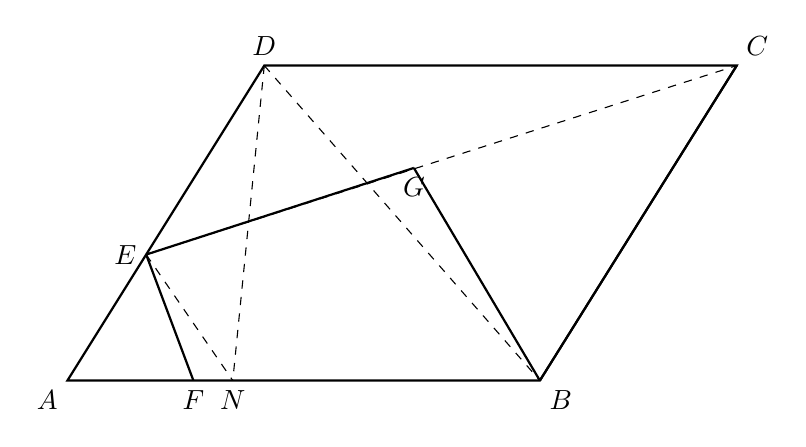
\begin{tikzpicture}
\coordinate (A) at (0,0);
\coordinate (B) at (6,0);
\coordinate (C) at (8.5,4);
\coordinate (D) at (2.5,4);
\coordinate (E) at (1.0,1.6);
\coordinate (F) at (1.6,0);
\coordinate (N) at (2.1,0);
\coordinate (G) at (4.4,2.7);

\draw[thick] (A) -- (B) -- (C) -- (D) -- cycle;
\draw[thick] (E) -- (F);
\draw[thick] (E) -- (G);
\draw[thick] (G) -- (B);
\draw[thick] (C) -- (B);

\draw[dashed] (D) -- (B);
\draw[dashed] (D) -- (N);
\draw[dashed] (E) -- (N);
\draw[dashed] (E) -- (C);

\node[below left] at (A) {$A$};
\node[below] at (F) {$F$};
\node[below] at (N) {$N$};
\node[below right] at (B) {$B$};
\node[left] at (E) {$E$};
\node[below] at (G) {$G$};
\node[above] at (D) {$D$};
\node[above right] at (C) {$C$};
\end{tikzpicture}
\end{document}
